
\newcommand{\wallH}{0.8} % = wall height
\newcommand{\lineW}{8} % = line width
\newcommand{\lineH}{0.6} % = line height diff
\newcommand{\size}{2.3} % Tjocklek på linjerna


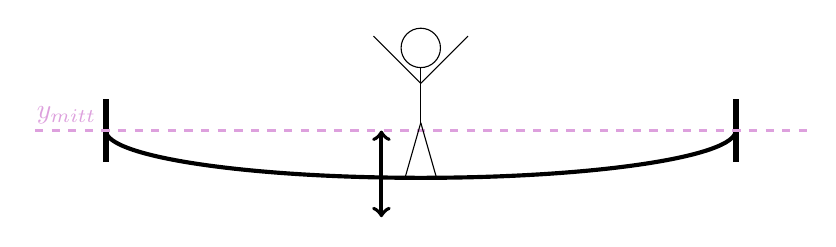
\begin{tikzpicture}

% Två raka sträck som håller i linan
\draw [line width=\size] (0,0) -- (0,\wallH);
\draw [line width=\size] (\lineW,0) -- (\lineW,\wallH);


% Själva linan
\draw [line width=1.5] (0,\wallH/2)  arc[x radius=\lineW/2, y radius=\lineH, start angle=180, end angle=360];

% Mittlinje
\draw [Plum,line width=1.2, dashed] (-0.9, 0.4) -- (\lineW+0.9,0.4);
\node [left, Plum] at (0, 0.6) {$y_{mitt}$};

% Ben
\draw (\lineW/2-0.2,-0.2) -- (\lineW/2,0.5);
\draw (\lineW/2+0.2,-0.2) -- (\lineW/2,0.5);

% Kropp
\draw (\lineW/2,0.5) -- (\lineW/2,1.2);

% Armar
\draw (\lineW/2-0.6,1.6) -- (\lineW/2,1);
\draw (\lineW/2+0.6,1.6) -- (\lineW/2,1);

% Huvud
\draw (\lineW/2, 1.45) circle [radius=0.25];


% Pil
\draw [<->, line width=1.4] (\lineW/2-0.5, 0.4) -- (\lineW/2-0.5, -0.7);


\end{tikzpicture}